\subsection{Cross Products}
\noindent
A cross product is a way of multiplying two vectors so that the result is a vector. Although the cross product technically only works for 3D vectors, we will first look a a "fake" 2D version to build an intuition.\\
$\vec{a}\times\vec{b}=a_1b_1-a_2b_2$. This "fake" 2D cross product gives the area of the parallelogram spanned by $\vec{a}$ and $\vec{b}$.\\
$\vec{a}\times\vec{b}=\norm{\vec{a}}\norm{\vec{b}}\sin{\theta}$ where $\theta$ is the angle between $\vec{a}$ and $\vec{b}$.\\
Another way to think of the magnitude of the cross product, both in 2D and 3D, is as a measure of how perpendicular two vector are.

\begin{figure}[h]
	\centering
	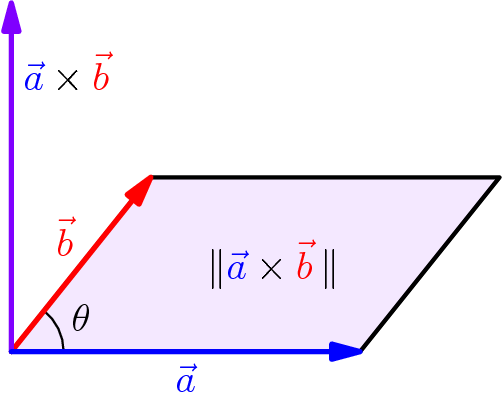
\includegraphics[scale=0.33]{Images/backgroundReview/CrossProduct}
\end{figure}


\noindent
In 3D, $\vec{a}\times\vec{b}$ is a vector, and similar to the 2D case, the magnitude of $\vec{a}\times\vec{b}$ is equal to the area of the parallelogram spanned by $\vec{a}$ and $\vec{b}$.\\
$\vec{a}\times\vec{b}=\langle a_2b_3-b_2a_3,a_3b_1-b_3a_1,a_1b_2-b_1a_2 \rangle$ and $\norm{\vec{a}\times\vec{b}}=\norm{\vec{a}}\norm{\vec{b}}\sin{\theta}$ where $\theta$ is the angle between $\vec{a}$ and $\vec{b}$.\\
Each component of $\vec{a}\times\vec{b}$ gives the area of the parallelogram spanned by $\vec{a}$ and $\vec{b}$ in some plane: The x-component of $\vec{a}\times\vec{b}$ gives the area in the yz-plane (x=0 plane).\\
$\vec{a}\times\vec{b}$ is perpendicular, also called "normal," to the plane containing $\vec{a}$ and $\vec{b}$. It's direction, is determined by the right hand rule.\\

\noindent
The cross product table of the standard basis vectors is useful for providing some insight into the properties of the cross product.
\begin{table}[h]
	\centering
	\begin{tabular}{|l|l|l|l|}
		\hline
		$\overrightarrow{\text{row}}\times\overrightarrow{\text{col}}$ & $\hat{i}$  & $\hat{j}$  & $\hat{k}$  \\ \hline
		$\hat{i}$                                & $0$        & $\hat{k}$  & $-\hat{j}$ \\ \hline
		$\hat{j}$                                & $-\hat{k}$ & $0$        & $\hat{i}$  \\ \hline
		$\hat{k}$                                & $\hat{j}$  & $-\hat{i}$ & $0$        \\ \hline
	\end{tabular}
\end{table}

\begin{itemize}
	\item NOT Commutative, but is antisymmetric: $\vec{a}\times\vec{b}=-\left(\vec{b}\times\vec{a}\right)$
	\item Scalar Associative: $\left(c\cdot\vec{a}\right)\times\vec{b}=\vec{a}\times\left(c\cdot\vec{b}\right)$
	\item Distributive: $\vec{a}\times\left(\vec{b}\times\vec{c}\right)=\vec{a}\times\vec{b}+\vec{a}\times\vec{c}$
\end{itemize}

\noindent
One can also think of the cross product as the determinant of a matrix.\\
\begin{center}
	$\vec{a}\times\vec{b}=\left|\begin{matrix}\hat{i}& \hat{j} & \hat{k} \\a_1 & a_2 & a_2\\b_1 & b_2 & b_3 \end{matrix}\right|$
\end{center}